	\subsection{Ajustement de la difficulté}
Il est nécessaire d'adapter la difficulté pour chaque joueur pour garantir une expérience de jeu optimale.			
\begin{quote}Malone : “Pour être stimulant, un jeu doit proposer un but que le joueur n’est pas certain d’atteindre”.
\end{quote}

	\subsubsection{Objectifs et paramètres d'ajustement}
L’objectif de l’ajustement de la difficulté est de pouvoir faire correspondre la difficulté du jeu aux capacités et niveau de jeu du joueur, de manière à ce que quel que soit son niveau, le feedback difficulté puisse être identique. Dans leur ouvrage \emph{On Game Design} \cite{Andr03} Andrew Rollings et Ernest Adams précisent cependant que l’ajustement ne doit pas être trop évident ni visible, afin d’éviter toute forme d’exploit, évidemment non voulu. Ils précisent aussi que cet ajustement ne doit pas se faire au détriment de l’impact décisif de l’action du joueur ; celui-ci doit rester le facteur décisif de sa réussite ou non, indépendemment de l’ajustement réalisé par le système. On pourra noter qu’un niveau de difficulté idéal mènerait le joueur à un taux d’échecs/réussites de 50/50.

		\paragraph{\emph{Évaluation de la difficulté}\\ \quad}
Modifier la difficulté d'un jeu vidéo ne semble pertinent qu'après en avoir évaluer le niveau lors de phases de tests. Deux types de tests peuvent être mis en place. 
\begin{itemize}
	\item des tests de jouabilité, réalisés par des joueurs testeurs : fidèles mais couteux et complexes à mettre en place, définis dans le temps et subjectifs.
	\item des tests par joueur synthétique : rapides, peu chers et répétables mais basiques, sans perception subjective, ignorent les aspects perceptifs.
\end {itemize} 

	\paragraph{\emph{Jeux de progression VS jeux d’émergence} \\ \quad}
Les jeux de progression sont scénarisés et le level design est défini et fixé à l’avance. La difficulté y est donc statique et prédéfinie selon les choix des designers. L’ensemble des situations du jeu a été pensé et calibré. Le parcours est relativement contraint et organisé. \\
Dans les jeux émergents, on ne peut prévoir l’évolution de la partie. Seul un certain nombre de règles permet de définir et de faire évoluer le contenu du jeu par application de ces règles et de l’interaction du joueur avec les objets du jeu. \\
Progression et émergence constituent en fait les deux formes opposées d’une catégorie décrivant le contrôle que possède le level designer sur l’expérience du joueur. On remplacera alors le contrôle manuel des designer par des algorithmes de génération appropriés. Un jeu pourra ainsi se situer le long de l’axe décrivant ce contrôle selon sa conception du level design (figure \ref{axe_scenaristique}). 
\begin{figure}[hbtp]
\centering
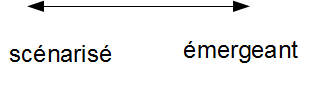
\includegraphics[width=5cm]{images/axe_scenaristique.png}
\caption{Axe scénaristique d'un jeu vidéo}
\label{axe_scenaristique}
\end{figure}

\paragraph{}Il existe un sous domaine de l’intelligence artificielle qui cherche à lier contenus émergents et scénarisés afin de tirer parti des avantages respectifs de l’un et l’autre domaine tout en limitant leurs contraintes : la narration interactive. On cherche alors à créer un univers virtuel où l’on va pouvoir “aller n’importe où et faire n’importe quoi, quand on le souhaite” de manière cohérente à la fois d’un point de vu gameplay et scénario. Cela en adaptant par exemple le scénario en fonction du comportement du joueur (utilisation par exemple d’un Drama Manager).

			\paragraph{\emph{Scénarisation VS adaptation dynamique} \\ \quad}
Le problème de l’adaptation de la difficulté est abordable à partir de deux méthodes de game design : la scénarisation et l’adaptation dynamique de la difficulté.  Ces deux méthodes pourraient bénéficier d’une méthode générale de la mesure de la difficulté, pour s’adapter au mieux.

\paragraph{}La scénarisation est une manière d’encadrer l’apprentissage du joueur à l’aide d’un découpage du gameplay en phases successives. 

\paragraph{}L’adaptation dynamique permet de maintenir le niveau de difficulté du jeu cohérent avec les capacités du joueur. Ces méthodes d’auto-adaptation peuvent être très efficaces, notamment pour ajuster un certain nombre de paramètres. Des algorithmes peuvent ainsi restreindre la lisibilité du jeu ou relâcher les contraintes de réalisation d’une action en fonction des résultats du joueur. On peut alors soit jouer sur la difficulté de la tâche ou de l’action à réaliser, soit sur les moyens employables pour y arriver (vie, temps, capacités, temps de réaction, propriétés du joueur / de l’environnement, etc.). Attention tout de même à ne pas faire un “système parfait” qui ferait que le joueur ne serait alors plus le facteur déterminant de sa réussite.

		\paragraph{\emph{Équilibrage dynamique} \\ \quad}
L’équilibrage dynamique, ou ajustement dynamique, consiste à modifier un certain nombre de paramètres du gameplay afin de s’adapter au comportement du joueur [Levieux, 11]. Il faut cependant pour cela d’abord être capable d’évaluer l’équilibre du jeu, sans quoi toute modification serait infondée . Dans cet objectif, l’apprentissage dynamique est particulièrement exploré. Ces techniques permettent en effet de calculer automatiquement les meilleurs paramètres pour atteindre un but donné, la difficulté du gameplay en l'occurrence. Idéalement, le jeu serait ainsi capable de détecter quand et comment le joueur parvient à surpasser les obstacles qui lui sont proposés, puis d’y répondre en proposant des modifications visant à obliger le joueur à reconsidérer sa stratégie de jeu. Bien sur, il est possible que le système ne parvienne pas à détecter la stratégie (voir l’exploit) du joueur, ou soit incapable de fournir une réponse appropriée ou cohérente avec l’univers du jeu, d’un point de vue autre que le gameplay pur. En effet, de tels systèmes ne prennent pas en compte l’intégralité de la pensée du game designer, qui reste complexe et non entièrement formalisable (visée artistique, morale, intentions, proposition d’une ‘expérience’ de jeu, etc.).

\paragraph{}Un jeu est donc une activité qui demande un effort au joueur. Cet effort librement consenti par le joueur  doit être utile pour la réussite ou non à ce jeu, puisqu’il pourrait aisément être rendu vain ou superflu en modifiant les règles du jeu. La difficulté, définie comme l’effort réalisé par le joueur, est donc une composante essentielle du jeu de part sa relation avec le joueur.

		\subsubsection{Techniques d'adaptation dans les jeux ludiques et sérieux}
L'adaptation de la difficulté dans les jeux vidéo est une fonctionnalité importante qui permet d’individualiser et de contextualiser l'expérience de jeu. Dans le cas de serious games, elle permet également de gérer la frustration des joueurs-apprenants tout en augmentant leurs motivations [Hocine et al 11]. L'individualisation et la contextualisation du jeu pour chaque joueur-apprenant, notions déjà définies par [Gee, 05] comme importantes pour l'apprentissage, ont pour conséquence d'augmenter sa satisfaction tout en améliorant l’efficacité de la formation.
				
		\paragraph{}
La génération dynamique d’IA permet de modifier le niveau de difficulté en créant de nouvelles entités avec un niveau et des règles donnés, ou en modifiant des paramètres du gameplay en cours de jeu.\\
Par exemple, Andrade et al utilisent l’apprentissage dynamique pour ajuster la difficulté. L’algorithme consiste à utiliser une base de couples (action, état de jeu) associés chacun à une valeur d’efficacité, afin que le jeu choisisse pour chaque situation un comportement de l’efficacité souhaitée.			
				
		\paragraph{\emph{Systèmes adaptables VS systèmes auto-adaptatifs} \\ \quad} 
L’adaptation peut être définie comme une caractéristique exprimée au niveau d’un système, dans notre cas un système informatique, qui reflète sa capacité à se modifier structurellement en réaction à certains évènements bien identifiés (Andresen K. et al, 2005). Nous parlerons de système adaptable lorsque l’intervention humaine est nécessaire pour enclencher le processus de modification et de système auto-adaptatif si aucune intervention extérieure n'est nécessaire (Moisuc B., 2001)

\paragraph{}
Levieux précise que la génération dynamique d’IA permet de modifier le niveau de difficulté en créant de nouvelles entités avec un niveau et des règles donnés, ou en modifiant des paramètres du gameplay en cours de jeu.\\
Par exemple, Andrade et al utilisent l’apprentissage dynamique pour ajuster la difficulté. L’algorithme consiste à utiliser une base de couples (action, état de jeu) associés chacun à une valeur d’efficacité, afin que le jeu choisisse pour chaque situation un comportement de l’efficacité souhaitée.

		\paragraph{\emph{Adaptation de la difficulté dans les jeux sérieux} \\ \quad}
Contribuer à l'acceptation et à l'utilisation des jeux sérieux constitue un enjeu majeur pour la réussite et l'efficacité de ceux-ci. En effet, ces systèmes sont destinés à satisfaire les joueurs-apprenants et à répondre à leurs besoins en termes d'acquisition de compétences et/ou de divertissement. L’adaptation a pour but d’améliorer l’utilisabilité d’un jeu sérieux ou ludique en restructurant certaines de ses propriétés.

\paragraph{}
[Hocine et al, 11] se proposent d'étudier les différents systèmes d'adaptation dans les jeux ludiques et sérieux. Pour évaluer ces systèmes, ils définissent trois critères majeurs :
\begin{itemize}
	\item L’efficacité d’un système évalue le degré de succès avec lequel les utilisateurs réalisent leurs objectifs dans le système.
	\item L’efficience évalue les moyens mis en œuvre par les utilisateurs pour accomplir leurs objectifs.
	\item La satisfaction évalue le niveau d’acceptation par les utilisateurs.
\end{itemize}

\paragraph{}
Afin d'évaluer et de comparer les différents systèmes, ils utilisent un système d'évaluation des techniques d'adaptation intéressant et très parlant du fait qu'il repose sur un modèle MVC (voir figure \ref{criteres_adaptation}).

\begin{figure}[!hbtp]
	\centering
	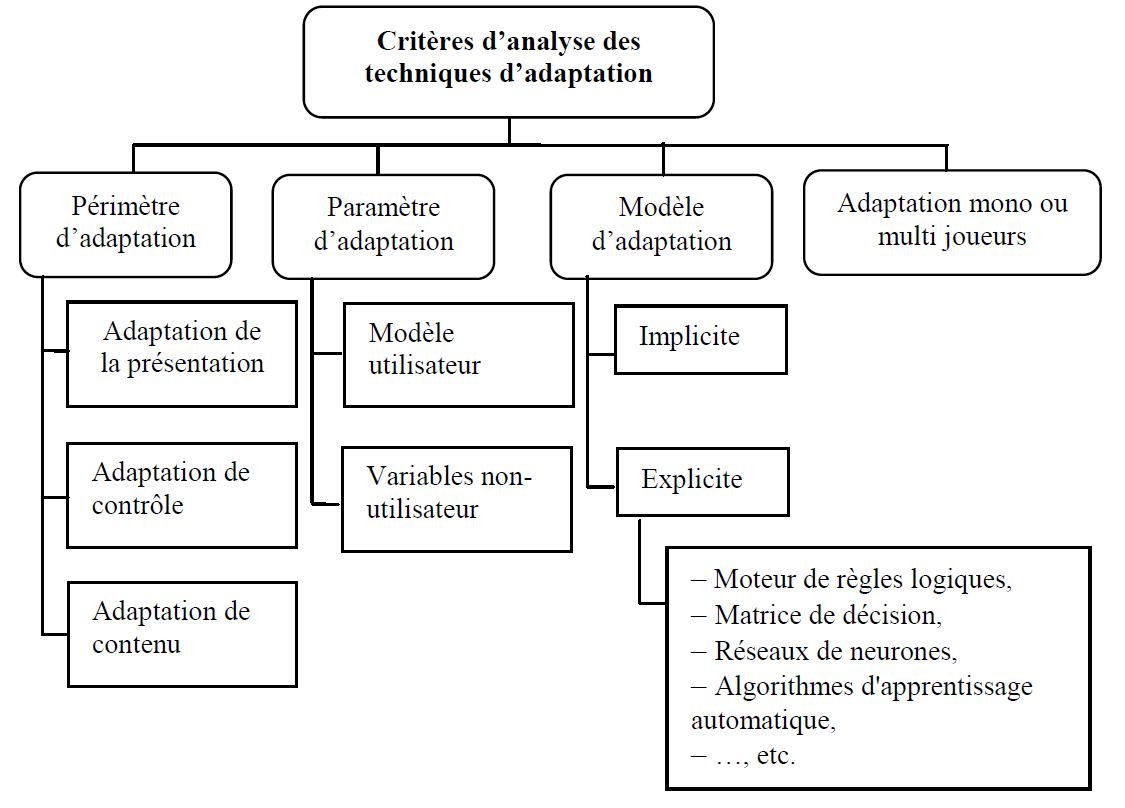
\includegraphics[width=1\linewidth]{images/criteres_adaptation.png}
	\caption{Critères d’analyse des techniques d’adaptation [Hocine et al, 2011]\cite{Hoci11}}
	\label{criteres_adaptation}
\end{figure}

	\paragraph{Périmètre d'adaptation\\}
Le périmètre de l'adaptation identifie le périmètre dans lequel l'adaptation est appliquée, selon le modèle MVC. 
\begin{itemize}
	\item \emph{Adaptation de la présentation (la Vue)}. L'adaptation peut donc avoir lieu au niveau de l'interface, du son ou de feedbacks envers l'utilisateur. Dans Hammer \& Planks, nous avons ainsi rendu possible la modification de ces paramètres : ajustement du volume de la musique ou des bruitages, contraste, taille des objets, vitesse de jeu et possibilité de désactiver les éléments cosmétiques facultatifs au jeu (animation de la mer, effets visuels etc.).
		\item  \emph{Adaptation du contrôle} : ce niveau englobe les règles du jeu et les règles métier qui spécifient la dynamique du jeu (ou le gameplay) en réaction aux actions des joueurs. C'est dans ce niveau que l'on adaptera le niveau de difficulté du jeu. Suite à mon travail sur le jeu Hammer \& Planks, il est possible de modifier le nombre et le type d'ennemis que doit affronter le joueur, la vitesse du jeu, les propriétés des personnages (joueur ou ennemis) ou encore la fréquence des obstacles par exemple.
		\item  \emph{Adaptation du contenu (le Modèle)} : l'adaptation à ce niveau modifie dynamiquement soit les schémas de données utilisés ou bien le contenu. L'adaptation s'efforce donc de produire un contenu lié au contexte de jeu et aux compétences des joueurs. Nous pouvons citer à titre d'exemple la génération automatique des dialogues et textes narratifs (Barry G., 2007) ou d'ambiance sonore (Chen Y et al, 2006)
\end{itemize} 

	\paragraph{Paramètres d'adaptation\\}
Ce sont les éléments sur lesquels repose la prise de décision du processus d'adaptation. Ces éléments vont être utilisés soit comme déclencheurs de l'adaptation soit comme sources de données. Hocine et al distinguent deux types de paramètres en fonction de l'utilisateur~:
\begin{itemize}
	\item \emph{Modèle utilisateur} : ensemble de variables et métriques décrivant les caractéristiques de l’utilisateur dans le système. Ces caractéristiques peuvent être des données représentant les préférences de l’utilisateur, son état attentionnel, ses émotions et/ou ses compétences. Ces données sont stockées dans le profil de l’utilisateur qui sera utilisé comme paramètre de processus d’adaptation.
	\item \emph{Paramètre non-utilisateur ou variable système }: ce paramètre représente les variables propres au système et qui ne dépendent pas du modèle utilisateur. A titre d'exemple, nous pouvons citer les paramètres liés à la configuration matérielle et logicielle du système hôte.
\end{itemize}

	\paragraph{Modèle d'adaptation\\}
	L’adaptation peut être implémentée dans le système sous forme d’un module qui interagit avec le système pour modifier son comportement et sa structure. Ce module peut être~:
\begin{itemize}
	\item \emph{Implicite} : dans ce cas les procédures d'adaptation se retrouvent éparpillées et étroitement liées aux différents composants du système. Il serait dans ce cas difficile de séparer dans les instructions (ou le code source) les éléments qui incombent à l'adaptation des autres aspects.
	\item \emph{Explicite }: la technique d'adaptation utilise des modèles explicites comme un moteur de règles logiques, une matrice de décision ou des algorithmes d’IA.
\end{itemize}
	
	\paragraph{Adaptation Mono ou Multi-joueurs\\}
Contrairement aux jeux mono-joueur, l'adaptation dans un système multi-joueurs doit prendre en compte l'aspect collaboratif et l'hétérogénéité entre les joueurs tout  en maintenant une cohérence globale du jeu.
	
	\paragraph{\emph{Tour d'horizon de systèmes d'ajustement dynamiques dans les jeux vidéo}	 \\ \quad}
Durant son travail sur la difficulté dans les jeux vidéo, Levieux se propose d'étudier les différentes solutions d’équilibrage dynamique qui ont été mis en place dans le jeu vidéo. Bien que de tels systèmes, de part leur aspect automatique, ne nous seront pas directement utiles, il peut être intéressant d'en connaître les principales mises en œuvre. On distingue plusieurs types de solutions~: 
\begin{enumerate}
	\item l’apprentissage par renforcement [Sutton 98]~:
	\begin{itemize}
		\item jeux de combat : [Andrade 05], [Graepel 04]
		\item RTS : [Madeira 04], [Madeira 06], [Ula 05]
		\item FPS : [Lee-Urban 08]
	\end{itemize}
	\item le scripting dynamique, qui calcule des préférences à partir de règles écrites par le designer~:
	\begin{itemize}
		\item jeux d’aventure : Neverwinter Nights - Bioware
		\item RTS : Wargus [Spronck 05], [Spronck 06], [Spronck 08], [Timuri 07], [Ludwig 07]
	\end{itemize}
		\item évolution génétique et réseau de neurones (l’un et/ou l’autre)~:
	\begin{itemize}
		\item jeux d’actions [Demasi 05], [Spronck 02]
		\item RTS : [Ponsen 05], [Agogino 00]
		\item FPS : [Cole 04], [Thurau 03]
		\item jeux de sport : Fifa 99 -EA Games [Chan 04]
		\item puzzle : Tetris - Nintendo [Bohm 05]
		\item réalité virtuelle : [Yannakakis 09], [Yannakakis 07]
	\end{itemize}
		\item algorithmes de champs potentiels pour comportements stratégiques dans les FPS [Thurau 04]
		\item raisonnement au cas par cas dans les RTS : [Aha 05]
\end{enumerate}

	\subsubsection*{Comparaison avec les besoins de NaturalPad}
Dans leur état de l'art des techniques d'adaptation dans les jeux vidéo, [Hocine et al] définissent la différence entre les systèmes adaptables et les systèmes auto-adaptatif. Leur étude, comme celle de Levieux, se concentrent cependant sur les systèmes dont l'ajustement est automatique. Or, comme nous l'avons déjà dit, nos besoins et propositions sont plutôt de proposer des jeux mettant en place un système d'ajustement manuel. Un tel système permet à chaque thérapeute amené à utiliser un jeu sérieux pour la santé de notre environnement, d'adapter le jeu aux besoins thérapeutiques dont il aura précisément besoin selon le contexte : préférences thérapeutiques, pathologies et spécificités du patient ou encore état de santé ou de forme de celui-ci pour ne citer que quelques exemples.